% !LW recipe = latexmk (xelatex)
\documentclass[12pt,a4paper,UTF8]{ctexart}
\usepackage{SJTUReport}
\usepackage{booktabs} % 三线表
\usepackage{amsmath}
\usepackage{amssymb}

%%-------------------------------正文开始---------------------------%%
\begin{document}

% %-----------------------封面--------------------%%
\cover

%------------------摘要-------------%%
\newpage
\begin{abstract}

在此填写摘要内容

\end{abstract}
\newpage

\thispagestyle{empty} % 首页不显示页码

%%--------------------------目录页------------------------%%
\newpage
\tableofcontents

%%------------------------正文页从这里开始-------------------%
\newpage

%可选择这里也放一个标题
\begin{center}
   \title{ \Huge \textbf{{考虑异质用户的高速公路换电站运营 MPC-RL 分层协同优化}}}
\end{center}


\section{Introduction}
随着电动汽车在高速公路中长距离出行场景中的普及，沿线补能设施的运营能力逐渐成为影响用户出行可靠性与系统运行效率的关键因素。相比传统充电方式，换电模式能够显著缩短车辆补能时间，但其运营过程同时受到用户需求、电池库存状态及电价变化等因素影响。【高速公路用户通常沿既定高速区间连续向下游行驶，驶过某一出口或换电站后难以折返，因此每一次站点选择都会改变后续可达站点集合；与此同时，不同车辆的到达 SOC 又会改变其首个可达站点以及整条换电站序列。】(前面的分析写得不够好，逻辑不够清晰，没有体现出高速换电场景的核心特点。应该是在高速场景下，长途出行的用户往往需要经历多次换电过程，每次换电行为具有相关性。然后解释如何相关。此外，每个用户车辆具有不同的SOC，SOC通过影响用户的续航里程进而影响用户的换电策略及站点的电池库存状态)。因此，高速公路换电站运营是一个复杂的、具有用户车辆电池状态和多站点电池状态时空耦合、动态演化特征的序贯决策问题。

在实际运营中，系统中存在两类异质用户：预约用户和随机到达用户。预约用户在运营日前提交计划到达高速入口的时间、行程起点和终点以及到达 SOC，运营者据此为用户提供换电路径，并提前规划站内电池充电计划以提高服务确定性；随机用户的到达时间和到达 SOC 则具有更强的不确定性，其可服务量取决于现场站点在优先履行预约服务后剩余的满电电池数量。预约用户的实际到达高速入口时间和到达 SOC 也可能偏离其提交的信息，因此运营者需要在用户实际到达高速入口时，根据预约用户和随机用户的最新到达情况、未来随机需求预测信息和站内库存动态情况调整其换电路径，来进一步提高服务质量和运营效率。考虑到分时电价进一步使站内充电成本随时间变化，如何协调预约用户履约、随机用户接纳以及站内电池充电调度，是高速公路换电网络运营中的核心问题。

针对上述问题，本文构建 MPC-RL 分层协同优化框架。换电站的实时运营中存在两类性质不同但相互耦合的决策：一类是预约用户换电路径指派动态调整决策，即根据每位用户的实际到达高速入口时间和 SOC，调整其相对于日前基准方案的换电站序列；另一类是各站逐块电池的连续充电功率决策。预约路径调整具有离散组合结构，并同时受到车辆续航、路径连通性、预约履约和多站点库存约束；随机需求预测与实际到达又会随时间不断更新。模型预测控制（Model Predictive Control, MPC）能够在有限预测域内联合评估这些约束和未来库存影响，并在每次获得新观测后重新优化而只执行当前用户批次，因而适合处理该类动态路径调整问题。充电功率的影响则具有明显的跨时段累积性：当前功率不仅决定当期充电成本，还会改变未来各站点每块电池的 SOC、满电电池供给能力和后续服务水平。本文采用强化学习（Reinforcement Learning, RL）学习逐电池充电功率控制策略，使其能够在长期交互过程中根据需求、电价和电池状态自适应调整充电行为。如\autoref{fig:MPC-RL}所示，RL 层输出逐电池充电功率并影响 SOC 状态转移，MPC 层在给定功率序列下优化预约用户路径，随机用户服务量由预约履约后的剩余满电电池供给确定。

\begin{figure}[!htbp]
    \centering
    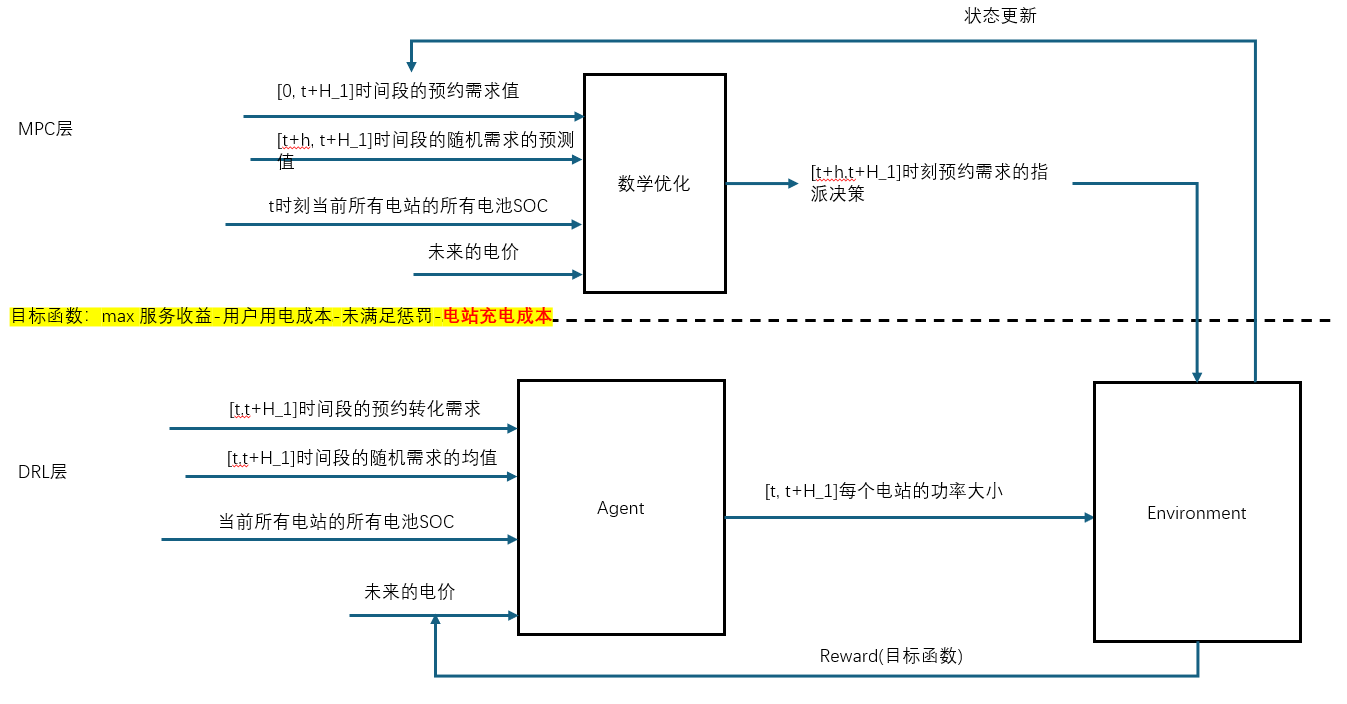
\includegraphics[width =1.0\textwidth]{figures/MPC-RL.png}
    \caption{MPC-RL协同优化框架（图中的随机需求均值是逐请求预测集合 $\widehat{\mathcal R}$ 的站点--时段聚合表示；随机实际到达通过状态更新反馈，未在图中单列；站级功率在数学模型中展开为逐电池连续功率向量）}
    \label{fig:MPC-RL}
\end{figure}


进一步地，本文利用 RL critic 提供预测时域之外的长期价值信息，以缓解有限预测时域导致的末端效应。传统 MPC 通常通过设置固定终端库存下界避免时域末端过度消耗满电电池，但该方法只能粗略限制末端满电电池数量，难以区分各站逐块电池 SOC 在未来需求和电价环境下的长期价值。本文在 RL 训练过程中学习状态价值函数，并在每轮 MPC 求解前计算 critic 对终端逐电池 SOC 的梯度，将其作为相应电池状态的长期边际价值。对于由当前预约指派产生但换电时刻位于预测域之外的履约需求，本文不额外训练新的 critic 分量，而是将其转化为“用归还电池的 SOC 替换一块满电电池”的等效终端影响。由此，RL 学到的长期电池状态价值被转化为 MPC 目标函数中的线性终端价值项。

因此，本文提出的 MPC-RL 框架基于决策属性进行分层：MPC 负责处理强约束、组合结构明显且需要可解释性的预约用户路径动态调整问题；RL 负责学习具有长期影响的逐电池充电功率策略，并通过 critic 向 MPC 提供终端 SOC 价值信息。二者通过逐电池 SOC 状态、连续充电功率决策、在途预约履约事件和终端价值项相互连接，从而在保证预约用户服务质量要求和运营约束可行性的同时，使有限时域 MPC 能够近似感知预测时域之外的长期影响。

本文其余部分安排如下：第 2 节给出问题描述与 MPC 模型，包括滚动时域机制、基于 SOC 分档的离线候选网络、日前基准路径和在线优化模型；第 3 节建立充电控制的马尔可夫决策过程并介绍 RL 算法；第 4 节和第 5 节分别给出实验分析和结论。全文将站点规定的服务就绪 SOC 归一化为 $1$；因此，“满电”表示达到该运营目标值，并不要求等于电芯的电化学上限。







\section{Problem Statement and MPC Formulation}

\subsection{Problem Statement}

考虑由多个 O-D 对及沿线换电站构成的单向高速公路换电网络。对于任一 O-D 对，车辆沿道路顺序向下游行驶且不能折返，一次长途行程可能需要在多个站点换电。每次换电都会从相应站点取走一块满电电池，并归还一块带有剩余电量的电池。因此，某位用户的站点选择不仅决定其后续可达站点，还会改变相关站点未来的电池库存，使用户路径与多站点库存产生时空耦合。

系统服务预约用户和随机到达用户。预约用户在运营日前提交预约信息，包括 O-D 对、预计进入高速公路的时刻及进入高速公路时的 SOC，运营者据此决定是否接受预约，并为已接受用户制定日前基准换电路径。当用户实际进入高速公路时，系统观测其真实进入时刻和 SOC，再根据实际情况为其调整路径。

随机到达用户在到达换电站时提出请求，并在预约需求得到满足后按先到先服务规则使用剩余满电电池。各站在每个时段内先充电、后换电，本时段退回的电池从下一时段开始充电。

运营者需要协调预约用户的换电路径与各站逐块电池的充电功率，从而在履行已接受预约的前提下，权衡换电收益、购电成本、路径调整成本和长期库存价值。本文采用分层 MPC--RL 框架：RL 根据需求、电价和库存状态生成预测时域内的充电功率，并向 MPC 提供终端库存价值；MPC 利用最新观测和随机需求预测，在逐电池库存时序约束下优化预约路径。

每轮优化后，系统仅发布本轮新进入用户的路径并执行下一时段的充电功率，随后根据实际到达和服务结果更新状态并重新求解。

\autoref{tab:notation}列出本节反复使用的核心符号。RL 的状态、动作和算法符号在第 3 节定义。

\begin{table}[!htbp]
  \centering
  \caption{MPC 模型的主要符号}
  \label{tab:notation}
  \scriptsize
  \setlength{\tabcolsep}{2pt}
  \renewcommand{\arraystretch}{0.88}
  \begin{tabular}{@{}lp{13cm}@{}}
    \toprule
    \textbf{符号} & \textbf{含义} \\
    \midrule
    \multicolumn{2}{l}{\textit{集合与索引}} \\
    $\ell,q$ & 当前滚动决策时刻和运行时段索引 \\
    $\mathcal{P},p$ & O-D 对集合及其索引 \\
    $\mathcal{K}^{p},k$ & O-D 对 $p$ 中已接受且已发布日前基准路径的预约用户集合及其索引 \\
    $\mathcal{K}_{\ell}^{\mathrm{arr},p},\mathcal{K}_{\ell}^{\mathrm{fut},p}$ & 本轮新进入高速公路的预约用户，以及预测时域内尚未进入的预约用户 \\
    $\mathcal{K}_{\ell}^{p}$ & 本轮参与路径优化的预约用户，$\mathcal{K}_{\ell}^{p}:=\mathcal{K}_{\ell}^{\mathrm{arr},p}\cup\mathcal{K}_{\ell}^{\mathrm{fut},p}$ \\
    $\mathcal{K}_{\ell}^{\mathrm{fix},p}$ & 本轮以前已进入高速公路、最终路径已发布且仍有换电事件尚未完成的预约用户 \\
    $\mathcal{T}$ & 决策时域内的运行时段集合，$\mathcal{T}:=\{\ell,\ldots,\ell+H\}$ \\
    $\mathcal{S}^{p},\mathcal{S}$ & O-D 对 $p$ 沿线的换电站集合，以及系统全部换电站的集合 \\
    $\mathcal{B}_{i},b$ & 站点 $i$ 的电池槽位集合及其索引 \\
    $\mathcal R_{i,q},\widehat{\mathcal R}_{i,q}$ & 时段 $q$ 实际到达站点 $i$ 的随机用户，以及时刻 $\ell$ 对该时段生成的虚拟随机请求 \\
    $\mathcal{V}^{p},n$ & O-D 对 $p$ 的节点集合及一般节点索引；节点包括入口 $o^p$、出口 $d^p$ 和换电站 $\mathcal S^p$ \\
    $\bar{\mathcal A}^{p,k},\mathcal A^{p,k}$ & 分别依据预约入口 SOC 和本轮有效入口 SOC 得到的个体可行弧集 \\
    \midrule
    \multicolumn{2}{l}{\textit{参数与状态}} \\
    $H$ & 预测时域长度 \\
    $t_A^{p,k},\bar t_A^{p,k}$ & 预约用户 $k$ 的实际入口时刻和最新计划入口时刻 \\
    $\mathrm{soc}_A^{p,k},\overline{\mathrm{soc}}_A^{p,k}$ & 预约用户 $k$ 的实际和预约入口 SOC \\
    $\widetilde t_{A}^{p,k},\widetilde{\mathrm{soc}}_{A}^{p,k}$ & 时刻 $\ell$ 采用的有效入口时刻和 SOC \\
    $q_{A,i}^{p,k}$ & 预约用户 $k$ 在本轮信息下到达节点 $i$ 的时段 \\
    $t_R^{i,u},\mathrm{soc}_R^{i,u}$ & 随机用户 $u$ 的实际到站时刻和 SOC \\
    $\widehat t_{R}^{i,\nu},\widehat{\mathrm{soc}}_{R}^{i,\nu}$ & 虚拟随机请求 $\nu$ 的预测到站时刻和 SOC \\
    $D_{i,j}^{p},D^{\mathrm{pref}}$ & 节点 $i$ 至下游节点 $j$ 的行驶距离，以及候选网络的期望换电间距 \\
    $v^{p}_{i,j}$ & 节点 $i$ 至 $j$ 的归一化 SOC 消耗 \\
    $\underline s_d^p,\tau_{p,i}$ & 到达出口的最低 SOC，以及从入口至节点 $i$ 的行驶时间 \\
    $\widehat P_{i,b,q}$ & RL 为槽位 $b$ 请求的充电功率 \\
    $e_{i,q},\pi_{i,q}^{\mathrm{sw}}$ & 时段 $q$ 的购电价格和单位换电电量服务价格 \\
    $E_B,\eta_i,\Delta$ & 额定电池能量、站点充电效率和固定时段长度 \\
    $\epsilon_{\mathrm{soc}},p_i^{\mathrm{tol}}$ & 满电补足的 SOC 容差及其在站点 $i$ 对应的功率余量 \\
    $\bar y_{A,i,j}^{p,k},y_{A,i,j}^{\mathrm{fix},p,k}$ & 日前基准路径和已发布的固定路径 \\
    $S_{i,b,q}^{\mathrm{obs}}$ & 时段 $q$ 结束后观测到的槽位 $b$ 的物理 SOC \\
    $\kappa>0,\beta\ge0$ & 路径调整惩罚和 RL 终端价值权重 \\
    \midrule
    \multicolumn{2}{l}{\textit{决策变量与主要辅助量}} \\
    $y_{i,j}^{p,k}$ & 预约用户 $k$ 是否经过可行弧 $(i,j)\in\mathcal A^{p,k}$ \\
    $\alpha_{i,b,\varepsilon,q}$ & 按规范化顺序连接换电事件与电池槽位的匹配辅助变量 \\
    $d_{p,k}$ & 路径差异指示量；在最优解中表示当前路径是否偏离日前基准路径 \\
    $z_{\nu,i,q}$ & 虚拟随机请求 $\nu$ 是否在本轮 MPC 预测轨迹中得到服务 \\
    $\delta_\varepsilon$ & 换电事件 $\varepsilon$ 是否在本轮 MPC 预测轨迹中激活 \\
    $P_{i,b,q}$ & 经满电补足与容量校正后的预测可行充电功率 \\
    $S_{i,b,q}^{\mathrm{pre}},S_{i,b,q}$ & 预测轨迹中槽位 $b$ 换电前和换电后的 SOC \\
    \bottomrule
  \end{tabular}
\end{table}



\subsection{MPC Formulation}
\subsubsection{Rolling-Horizon Information and Execution}


\begin{figure}[!htbp]
    \centering
    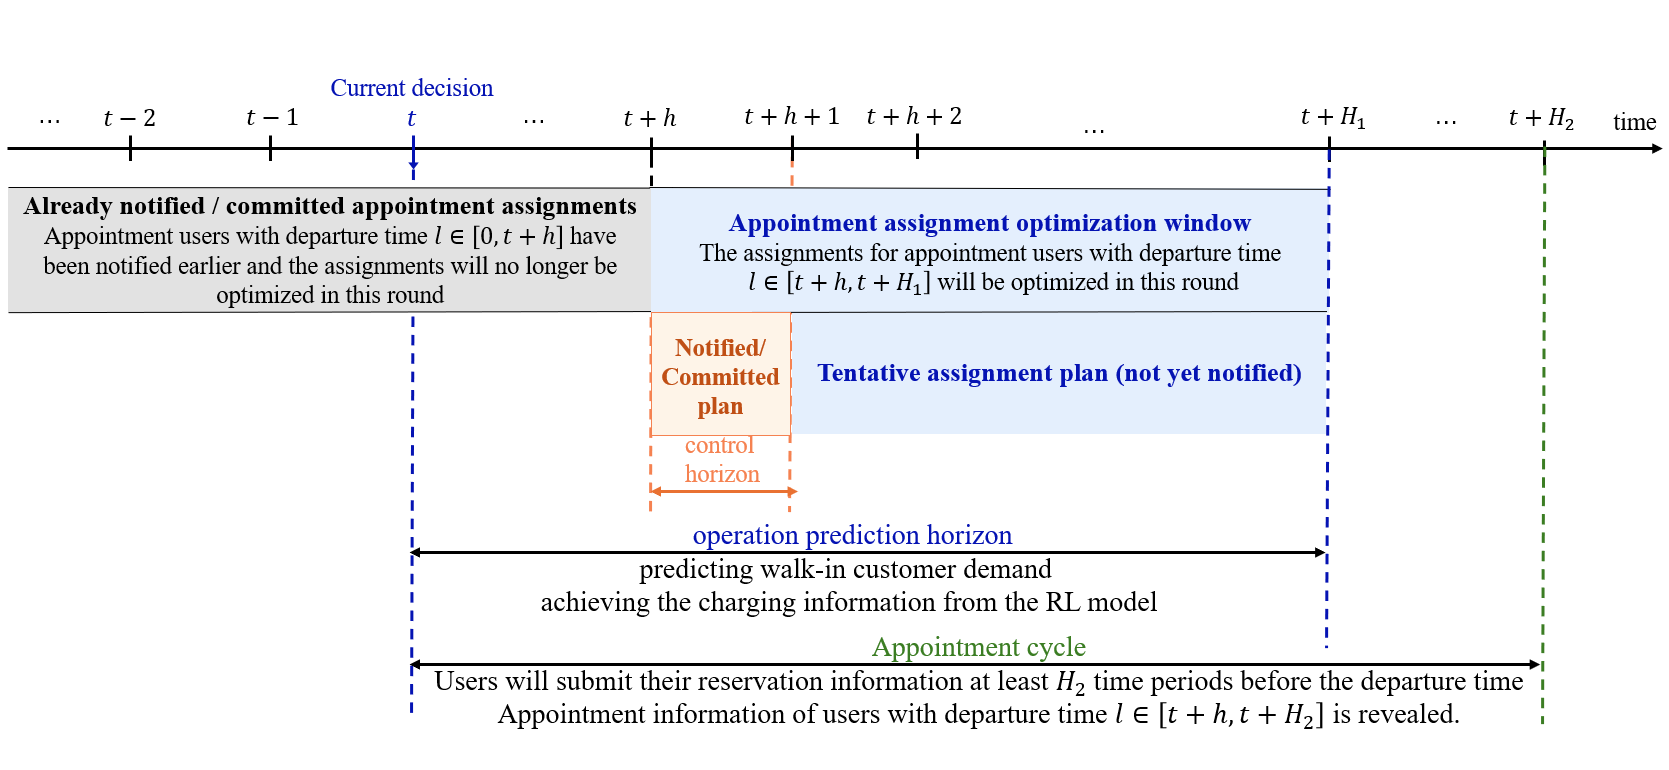
\includegraphics[width =1.0\textwidth]{figures/rolling_horizon.png}
    \caption{滚动时域内的信息更新、优化与首阶段执行}
    \label{fig:rolling_horizon}
\end{figure}


设当前滚动决策时刻为 $\ell$，预测时域包含未来 $H$ 个时段，决策时域为$\mathcal T=\{\ell,\ldots,\ell+H\}$。连续时刻落在区间 $[q,q+1)$ 时归入时段 $q$。

如\autoref{fig:rolling_horizon}所示，系统在时刻 $\ell$ 观测区间 $(\ell-1,\ell]$ 内新进入高速公路的预约用户和实际到达各站的随机用户，完成上一时段的物理状态更新。预约用户 $k$ 的实际到达入口时刻和 SOC 分别记为 $t_A^{p,k}$ 和 $\mathrm{soc}_A^{p,k}$；随机用户 $\nu$ 的实际到站时刻和 SOC 分别记为 $t_R^{i,\nu}$ 和 $\mathrm{soc}_R^{i,\nu}$。


运行过程中不再接受新的当日预约。对于未来时段，对尚未进入高速公路的预约用户，$\bar t_A^{p,k}$ 表示用户的日前预约到达时刻，$\overline{\mathrm{soc}}_A^{p,k}$ 表示用户的日前预约 SOC。对尚未到达的随机用户，$\widehat t_{R}^{i,\nu}$ 表示预测到站时刻，$\widehat{\mathrm{soc}}_{R}^{i,\nu}$ 表示预测到站 SOC。

对 O-D 对 $p$，令
\begin{align}
\mathcal K_{\ell}^{\mathrm{arr},p}
&=\left\{k\in\mathcal K^p:t_A^{p,k}\in(\ell-1,\ell]\right\},\\
\mathcal K_{\ell}^{\mathrm{fut},p}
&=\left\{k\in\mathcal K^p:k\text{ 尚未进入系统},
\ \bar t_A^{p,k}\in(\ell,\ell+H]\right\},\\
\mathcal K_{\ell}^{p}
&=\mathcal K_{\ell}^{\mathrm{arr},p}\cup\mathcal K_{\ell}^{\mathrm{fut},p}.
\label{eq:rolling_user_sets}
\end{align}
其中，$\mathcal K_{\ell}^{\mathrm{arr},p}$ 表示本轮新进入高速公路、因而已观测到实际信息的预约用户，$\mathcal K_{\ell}^{\mathrm{fut},p}$ 表示预计在预测时域内进入但尚未到达的预约用户。为统一两类用户在模型中的表达，定义本轮采用的有效入口信息
\begin{equation}
\left(\widetilde t_{A}^{p,k},
\widetilde{\mathrm{soc}}_{A}^{p,k}\right)=
\begin{cases}
\left(t_A^{p,k},\mathrm{soc}_A^{p,k}\right),
&k\in\mathcal K_{\ell}^{\mathrm{arr},p},\\
\left(\bar t_A^{p,k},\overline{\mathrm{soc}}_A^{p,k}\right),
&k\in\mathcal K_{\ell}^{\mathrm{fut},p}.
\end{cases}
\label{eq:effective_arrival_information}
\end{equation}
$\mathcal K_\ell^{\mathrm{fix},p}$ 仅包含更早时段已进入高速公路的用户，与 $\mathcal K_\ell^p$ 不重叠。求解后，系统只向 $\mathcal K_{\ell}^{\mathrm{arr},p}$ 中的本轮新进入用户发布路径；$\mathcal K_{\ell}^{\mathrm{fut},p}$ 的路径不对用户发布，仅用于前瞻评价。

对于站点 $i$，令
\begin{equation}
\mathcal R_{i,q}
\end{equation}

实际随机用户按其到站时刻归入 $\mathcal R_{i,q}$，预测请求按其预测到站时刻归入 $\widehat{\mathcal R}_{i,q}$。

系统随后执行时段 $\ell$ 的充电功率和换电服务。时段结束后，物理库存更新，未执行的未来预测也在下一滚动时刻重新生成。已发布但尚未完成的预约路径作为固定履约承诺进入后续模型。这一机制可概括为“滚动时域优化、首阶段执行”。

设 $\tau_{p,i}$ 为 O-D 对 $p$ 从入口到节点 $i$ 的行驶时间。预约用户 $k$ 到达节点 $i$ 的时段 $q_{A,i}^{p,k}=[\widetilde t_{A}^{p,k}+\tau_{p,i}]$，其中 $[\cdot]$ 表示向下取整运算。

当 $q_{A,i}^{p,k}\in\mathcal T$ 时，相应换电事件显式进入本轮逐电池 SOC 转移；当 $q_{A,i}^{p,k}>\ell+H$ 时，该事件“发出一块满电电池并接收一块具有相应 SOC 的退回电池”的影响通过 RL 终端价值项进行等效评价.


\subsubsection{Offline Candidate networks by SOC Range}

在上一小节我们介绍了滚动优化机制。在每个决策时刻，我们需要安排预测时域内每个预约用户的换电站序列。如何高效、清晰地表示解的结构，设计决策变量是我们首要考虑的问题。本文借鉴加油站选址模型中 expanded network 的思路，用一条入口--出口路径表示该序列：对于O-D pair $p$，若路径为
$o^p\rightarrow i_1\rightarrow\cdots\rightarrow i_r\rightarrow d^p$，则用户依次在换电站$i_1,\ldots,i_r$ 换电；一条弧跨过的沿线站点均不被访问。为避免在每个滚动时刻重复枚举全部下游组合，本文在运营前先生成一个候选路径网络。不同的用户出发SOC会影响车辆的续航里程，从而影响可达的换电站集合。我们将用户到达高速时的SOC划分为若干个离线区间，并在每个区间上生成相应的候选网络。

对每个 O-D 对 $p$，节点集合为
$\mathcal V^p=\{o^p\}\cup\mathcal S^p\cup\{d^p\}$。所有节点均按高速公路下游方向排列。参数 $D_{i,j}^p$ 和 $v_{i,j}^p>0$ 分别表示从 $i$ 到下游节点 $j$ 的行驶距离和 SOC 消耗。

考虑到现实场景中，为用户安排两个距离过近的连续站点换电是不合理的。同时也为了减少网络规模，我们给定一个最小换电间距 $\underline D>0$，生成的网络将在保证方案可行性的基础上，尽量排除从入口到首个换电站以及任意两个连续访问换电站之间距离小于 $\underline D$ 的方案。指向出口的末段行程不受该间距偏好约束，但车辆到达出口时的 SOC 不得低于 $\underline s_d^p$。

对每个 SOC 区间 $h$ 和 O-D 对 $p$，离线网络按以下步骤生成。

\begin{enumerate}
  \item[\textbf{Step 1.}] \textbf{生成原始弧。}若车辆以该 SOC 区间的上限电量能够从入口 $o^p$ 到达下游换电站 $j$，则连接二者；若 $v_{i,j}^p\le1$，则连接两个依次位于下游的换电站 $i$ 和 $j$；若 $v_{i,d^p}^p+\underline s_d^p\le1$，则连接换电站 $i$ 与出口 $d^p$。

  \item[\textbf{Step 2.}] \textbf{生成完整可行路径。}在原始网络中枚举所有从 $o^p$ 到 $d^p$ 的完整路径。

  \item[\textbf{Step 3.}] \textbf{剪枝过近换电弧。}从上述完整路径中找出距离小于 $\underline D$ 的入口--首站弧和站间弧，并按距离从小到大排序。依次考察每条过近弧，如果现有的完整路径中仍存在至少一条不包含该弧的方案，则删除该弧，否则保留。

  \item[\textbf{Step 4.}] \textbf{形成候选网络。}将最终保留的完整路径所包含的弧合并为 $\mathcal A^{h,p}$，候选网络由节点集 $\mathcal V^p$ 和弧集 $\mathcal A^{h,p}$ 组成。
\end{enumerate}


离线网络根据入口 SOC 直接选用。预约 SOC 所在区间对应的离线弧集作为候选弧集 $\mathcal A^{p,k}$.




\subsubsection{Day-Ahead Baseline Path Generation}

用户提交预约信息
$\left(p,\bar t_A^{p,k},\overline{\mathrm{soc}}_A^{p,k}\right)$
后，运营者依据其行程、预计入口时刻和入口 SOC 检查能否提供服务，并为可接受的请求生成日前基准路径。该路径在用户实际进入高速公路后仍可根据最新观测调整。

预约请求按提交顺序处理。处理当前请求前，算法根据已接受预约和日前随机需求预测，递推估计各站未来各时段的电池库存。部署时，日前充电功率由训练完成的同一 actor 的均值策略在日前预测状态上逐期生成，并采用与在线模型一致的满电补足和容量约束；因此，给定初始库存、需求预测和下述并列规则，日前库存递推与预约接纳结果可以复现。每个时段先更新充电结果，再扣除已安排的预约换电和预计的随机换电；本时段退回的电池从下一时段开始充电。

对 O-D 对 $p$ 的预约用户 $k$，基准路径按以下规则生成：
\begin{enumerate}
  \item 车辆从入口出发时的 SOC 为 $\overline{\mathrm{soc}}_A^{p,k}$，每次换电后恢复为 $1$。下一节点沿候选弧集 $\mathcal A^{p,k}$ 选择，因此首段和站间行程均满足续航要求。
  \item 若车辆能够从当前位置直接到达出口，且到达 SOC 不低于 $\underline s_d^p$，则下一站选择出口；否则，仅保留预计到站时有满电电池可用、并且仍存在可行下游延续路径的候选站。
  \item 候选站按预计满电电池余量从高到低排序，余量相同时优先选择更靠近出口的站点。选定站点后，在相应时段为该用户预留一块满电电池，并更新该站后续时段的预计库存；随后重复上述过程。
\end{enumerate}

若任一步不存在满足库存与下游可达性要求的候选站，则拒绝该请求；只有成功生成完整入口--出口路径的用户才进入 $\mathcal K^p$。对已接受用户，若基准路径经过弧 $(i,j)$，则令 $\bar y_{A,i,j}^{p,k}=1$，否则为 $0$。该路径随预约结果一并发布，并作为滚动优化的基准方案。


\subsubsection{Optimization Model}

给定时刻 $\ell$ 的观测库存、预约用户的有效入口信息、预测的未来随机需求和 RL 输出功率，MPC 调整预约路径。

\paragraph{Reservation-path variables.}
\[
y_{i,j}^{p,k}\in\{0,1\},
\qquad
(i,j)\in\mathcal A^{p,k}.
\]
若 O-D 对 $p$ 的预约用户 $k$ 经过弧 $(i,j)$，则
$y_{i,j}^{p,k}=1$。一组满足流平衡的 $y$ 变量唯一确定该用户依次访问的换电站序列。

\paragraph{Battery-matching auxiliary variables.}
将某一预约用户或预测随机请求在站点 $i$、时段 $q$ 发起的一次换电需求称为一个换电事件，并用 $\varepsilon$ 对事件进行编号。一个事件被激活，表示对应需求在本轮 MPC 轨迹中接受换电服务；三类换电事件及其激活规则将在约束 4 中统一定义。电池分配变量为
\[
\alpha_{i,b,\varepsilon,q}\in\{0,1\}.
\]
若站点 $i$ 的槽位 $b$ 在时段 $q$ 与换电事件 $\varepsilon$ 匹配，则
$\alpha_{i,b,\varepsilon,q}=1$；否则为 $0$。

模型还引入以下辅助变量。其中，
$z_{\nu,i,q}$ 表示预测随机请求 $\nu$ 是否在本轮 MPC 轨迹中被服务，其取值由预约履约后的剩余满电供给余量和先到先服务顺序确定；
$d_{p,k}$ 表示当前路径是否偏离日前基准路径；
$P_{i,b,q}$ 是对 RL 输出进行校正后的充电功率；
$S_{i,b,q}^{\mathrm{pre}}$ 和 $S_{i,b,q}$ 分别表示充电后换电前以及换电后的 SOC；
$g_{i,b,q}$ 和 $F_{i,q}$ 分别表示服务就绪指示量和可用电池数。

\textbf{Objective function}

本轮 MPC 的目标为最大化综合运营价值：
\begin{equation}
\max\quad
I^{\mathrm{MPC}}-C_{\mathrm{ch}}-C_{\mathrm{adj}}
+\beta\Phi^{\mathrm{RL}}.
\label{eq:objective}
\end{equation}
其中 $I^{\mathrm{MPC}}$、$C_{\mathrm{ch}}$、$C_{\mathrm{adj}}$ 和 $\Phi^{\mathrm{RL}}$ 分别表示换电服务收益、充电成本、路径调整成本和 RL 终端价值，下面分别给出其定义。

\paragraph{Swap-service revenue.}
令 $\pi_{i,q}^{\mathrm{sw}}\ge0$ 表示站点 $i$ 在时段 $q$ 的单位换电电量服务收费，单位为金额/电量。用户获得满电电池并退回 SOC 为 $\rho$ 的电池时，本次换电对应的服务电量为 $E_B(1-\rho)$。因此，预约用户收益与随机用户收益分别为
\begin{equation}
\begin{aligned}
I^{\mathrm{MPC}}&=I^{A}+\widehat I^{R},\\
I^{A}
&=E_B\sum_{q\in\mathcal T}
\sum_{i\in\mathcal S}\pi_{i,q}^{\mathrm{sw}}
\sum_{\varepsilon\in\mathcal E_{i,q}^{A,\mathrm{dec}}}
(1-\rho_\varepsilon)\delta_\varepsilon,\\
\widehat I^{R}
&=E_B\sum_{q\in\mathcal T}
\sum_{i\in\mathcal S}\pi_{i,q}^{\mathrm{sw}}
\sum_{\nu\in\widehat{\mathcal R}_{i,q}}
(1-\widehat{\mathrm{soc}}_{R}^{i,\nu})
z_{\nu,i,q}.
\end{aligned}
\label{eq:income}
\end{equation}
其中，$I^{A}$ 计入本轮路径决策产生的预约换电收益；已发布固定预约的收益与本轮决策无关，作为常数从目标函数中省略。$\widehat I^{R}$ 使用时刻 $\ell$ 的预测到站信息，因而是前瞻收益而非已实现收益。事件集合、激活量 $\delta_\varepsilon$ 和退回 SOC $\rho_\varepsilon$ 由约束 4 统一定义。个体可行弧集已规定车辆一旦能够满足出口 SOC 要求便直接驶向出口，因此正的服务收益不会诱导可避免的额外换电。

式\eqref{eq:automatic_random_service}强制服务所有有剩余电池可供满足的预测随机请求；真实随机服务收益在 RL 奖励中根据 $\mathcal R_{i,q}$ 和 $\mathrm{soc}_R^{i,u}$ 另行结算。

\paragraph{Charging cost.}
$P_{i,b,q}$ 是本轮 MPC 轨迹中包含必要满电补足的可行充电功率，相应的预测时域购电成本为
\begin{equation}
C_{\mathrm{ch}}
=
\sum_{q\in\mathcal T}
\sum_{i\in\mathcal S}
\sum_{b\in\mathcal B_i}
e_{i,q}\Delta P_{i,b,q}.
\label{eq:chargingcost}
\end{equation}
该项计入不同站点和时段的电价，以及预测轨迹内充入电量造成的运营支出；RL 奖励只结算首个执行时段的实际购电成本。

\paragraph{Path-adjustment cost.}
若预约用户的当前换电站序列不同于日前基准路径，则产生一次调整成本：
\begin{equation}
C_{\mathrm{adj}}
=
\kappa
\sum_{p\in\mathcal P}
\sum_{k\in\mathcal K_\ell^p}
d_{p,k}.
\label{eq:adjustment_cost}
\end{equation}
每名用户无论改变一个还是多个换电站均只计一次惩罚。$\mathcal K_\ell^{\mathrm{fut},p}$ 中未来用户的调整成本是前瞻成本；只有
$\mathcal K_\ell^{\mathrm{arr},p}$ 中本轮路径被正式发布的用户产生实际调整支出。

\paragraph{RL terminal value.}
有限预测时域会截断两类长期影响：域内决策在时刻 $\ell+H$ 留下的电池 SOC 会继续影响后续运营；本轮路径还可能包含到站时刻晚于 $\ell+H$ 的预约换电，这些事件尚未进入域内 SOC 转移，却会在未来消耗满电库存。为评价这两类影响，本文使用第 3 节训练的 critic $V_\theta$ 为 MPC 提供预计算的价值系数，而不将非线性网络直接嵌入优化模型。

每轮求解前，系统依据固定承诺、当前有效预约信息、随机需求预测和 actor 的均值动作生成一条与本轮路径变量无关的参考轨迹。固定承诺沿已发布路径执行；对 $\mathcal K_\ell^p$ 中的用户，系统在满足个体可达性和参考库存约束的名义路径组合中，先最小化相对日前基准的路径变更数，再按用户与弧编号作字典序选择。该确定性可行性计算与经济目标及本轮路径变量无关。本文假设已接受预约在允许的到达更新范围内至少存在一组这样的名义可行路径；若外生故障或极端偏差破坏该条件，则进入模型范围之外的应急履约机制。参考轨迹的终端状态记为 $s_{\ell+H}^{\mathrm{ref}}$。在该状态处，critic 对槽位 SOC 的边际价值为
\begin{equation}
\lambda^S_{i,b}
=
\left.
\frac{\partial V_{\theta}(s)}
{\partial S_{i,b}}
\right|_{s=s_{\ell+H}^{\mathrm{ref}}},
\quad i\in\mathcal S,\ b\in\mathcal B_i.
\label{eq:marginal_value_soc}
\end{equation}
$\lambda^S_{i,b}$ 表示参考状态附近单位 SOC 增量带来的长期价值。对 critic 作一阶近似并删除与本轮决策无关的常数后，域内终端库存只需保留线性项 $\lambda^S_{i,b}S_{i,b,\ell+H}$。

对于满足 $q_{A,i}^{p,k}>\ell+H$ 的预约换电，若入弧 $(j,i)$ 被选择，则站点 $i$ 将在预测时域外发出一块满电电池并接收 SOC 为 $\rho_{A,j,i}^{p,k}$ 的退回电池。该事件不改变域内终端 SOC，因而需要单独估值。为使反事实在参考终端库存暂时没有满电电池时仍有定义，在站点 $i$ 选择一个规范化槽位：若存在服务就绪槽位，则取编号最小者；否则取 SOC 最高者，并以最小编号打破并列。记 $s_{\ell+H}^{\mathrm{ref},(i,x)}$ 为仅将该槽位 SOC 置为 $x$、其余状态保持不变的参考终端状态，并定义
\begin{equation}
\Delta V_{i}^{\mathrm{out}}(\rho)
=
 V_\theta\!\left(s_{\ell+H}^{\mathrm{ref},(i,\rho)}\right)
-V_\theta\!\left(s_{\ell+H}^{\mathrm{ref},(i,1)}\right).
\label{eq:outside_swap_value}
\end{equation}
$\Delta V_{i}^{\mathrm{out}}(\rho)$ 在 MPC 求解前由 critic 计算，并作为路径变量的固定系数。当 $\rho<1$ 且 critic 合理反映库存价值时，该值通常为负，对应未来履约的库存机会成本。上述成对反事实比较的是同一规范化槽位从满电变为退回 SOC 的价值变化，不要求参考轨迹事先在该站保留满电电池；当所选槽位原本已满电时，$s_{\ell+H}^{\mathrm{ref},(i,1)}$ 即与原参考状态一致。

去除不影响最优解的常数项后，进入式\eqref{eq:objective}的 RL 终端价值为
\begin{equation}
\begin{aligned}
\Phi^{\mathrm{RL}}
={}&
\sum_{i\in\mathcal S}\sum_{b\in\mathcal B_i}
\lambda^S_{i,b}S_{i,b,\ell+H}\\
&+\sum_{p\in\mathcal P}
\sum_{k\in\mathcal K_\ell^p}
\sum_{i\in\mathcal S^p}
\sum_{\substack{j:(j,i)\in\mathcal A^{p,k}\\
q_{A,i}^{p,k}>\ell+H}}
\Delta V_{i}^{\mathrm{out}}\!\left(\rho_{A,j,i}^{p,k}\right)
y_{j,i}^{p,k}.
\end{aligned}
\label{eq:rl_terminal_value}
\end{equation}
第一项评价预测时域结束时的逐电池库存；第二项只在相应入弧被选择时计入尚未反映在终端 SOC 中的域外换电价值。域内换电已通过式\eqref{eq:continuous_swap_transition}进入第一项，固定承诺也已包含在参考状态中，因而均不重复计算。多个域外事件的价值采用可加近似，忽略其高阶交互；$\beta$ 用于校准 critic 价值与域内运营金额的尺度。

\textbf{Constraints}

\paragraph{Constraint 1: Reservation-path feasibility.}
每位预约用户满足以下流平衡约束：
\begin{equation}
\sum_{\{j\mid(n,j)\in\mathcal A^{p,k}\}}
y_{n,j}^{p,k}
-
\sum_{\{j\mid(j,n)\in\mathcal A^{p,k}\}}
y_{j,n}^{p,k}
=
\begin{cases}
1,&n=o^p,\\
-1,&n=d^p,\\
0,&n\in\mathcal S^p,
\end{cases}
\quad
p\in\mathcal P,\ k\in\mathcal K_\ell^p,\ n\in\mathcal V^p.
\label{eq:flow}
\end{equation}
入口净流出为 1、出口净流入为 1，中间节点流入等于流出，因此每名用户选择一条完整的入口--出口路径。变量只建立在在线可行弧集
$\mathcal A^{p,k}$ 上。

\paragraph{Constraint 2: Path-adjustment identification.}
定义当前路径和日前基准路径的站点访问指示量
\begin{equation}
x_{A,i}^{p,k}
=
\sum_{\{j\mid(j,i)\in\mathcal A^{p,k}\}}y_{j,i}^{p,k},
\qquad
\bar x_{A,i}^{p,k}
=
\sum_{\{j\mid(j,i)\in\bar{\mathcal A}^{p,k}\}}\bar y_{A,j,i}^{p,k}.
\label{eq:station_visit_indicator}
\end{equation}
并设置
\begin{subequations}
\label{eq:path_adjustment_indicator}
\begin{align}
d_{p,k}
&\ge x_{A,i}^{p,k}-\bar x_{A,i}^{p,k},
&&p\in\mathcal P,\ k\in\mathcal K_\ell^p,\ i\in\mathcal S^p,\\
d_{p,k}
&\ge \bar x_{A,i}^{p,k}-x_{A,i}^{p,k},
&&p\in\mathcal P,\ k\in\mathcal K_\ell^p,\ i\in\mathcal S^p.
\end{align}
\end{subequations}
只要当前路径增加或删除任意换电站，就有 $d_{p,k}=1$；完整换电站序列与日前基准一致时，在目标函数中的正调整成本作用下有 $d_{p,k}=0$。

\paragraph{Constraint 3: Feasible charging power and post-charge SOC.}
为使服务电池的物理 SOC 与模型中的满电 SOC $1$ 一致，站内控制器对接近满电的 RL 请求执行小幅补足。令 $0<\epsilon_{\mathrm{soc}}<1$ 为统一的满电补足容差，并令
$p_i^{\mathrm{tol}}=E_B\epsilon_{\mathrm{soc}}/(\eta_i\Delta)$
为该补足容差对应的功率余量。轨迹功率由以下两个闭合分支确定：
\begin{subequations}
\label{eq:power_saturation}
\begin{align}
g_{i,b,q}=0
&\Longrightarrow
\begin{cases}
P_{i,b,q}=\widehat P_{i,b,q},\\
\widehat P_{i,b,q}
\le \dfrac{E_B(1-S_{i,b,q-1})}{\eta_i\Delta}
-p_i^{\mathrm{tol}},
\end{cases}
\label{eq:defer_completion}\\
g_{i,b,q}=1
&\Longrightarrow
\begin{cases}
P_{i,b,q}
=\dfrac{E_B(1-S_{i,b,q-1})}{\eta_i\Delta},\\
\widehat P_{i,b,q}
\ge \dfrac{E_B(1-S_{i,b,q-1})}{\eta_i\Delta}
-p_i^{\mathrm{tol}}.
\end{cases}
\label{eq:complete_charging}
\end{align}
\end{subequations}
第一分支严格执行 RL 请求，并使电池与满电至少相差 $\epsilon_{\mathrm{soc}}$；第二分支把电池恰好补至 SOC $1$。补足功率不超过 $p_i^{\mathrm{tol}}$，并完整计入式\eqref{eq:chargingcost}的充电成本。两分支在请求恰好到达补足边界时均可选择，分别表示推迟完成和立即补足；二者对应不同的实际功率与 SOC，不产生能量记账缺口。日前递推和参考 rollout 在该边界固定采用立即补足分支，以保证参考轨迹唯一；在线 MPC 则保留两种物理可行动作，并将首期 $g^*$ 传递给执行层。式\eqref{eq:power_saturation}可直接写为求解器的线性 indicator 约束。只有 $q=\ell$ 的最优首项会被实际执行，其余时段仅用于前瞻评价。充电后的预测 SOC 为
\begin{equation}
S_{i,b,q}^{\mathrm{pre}}
=
S_{i,b,q-1}
+\frac{\eta_i\Delta}{E_B}P_{i,b,q},
\quad i\in\mathcal S,\ b\in\mathcal B_i,\ q\in\mathcal T.
\label{eq:continuous_charging_transition}
\end{equation}


\paragraph{Constraint 4: Swap events and service priority.}
用户 $k$ 沿入弧 $(j,i)$ 到达站点 $i$ 时，退回电池的 SOC 为
\begin{equation}
\rho_{A,j,i}^{p,k}
=
\begin{cases}
\widetilde{\mathrm{soc}}_{A}^{p,k}-v_{o^p,i}^{p},
&j=o^p,\\
1-v_{j,i}^{p},
&j\in\mathcal S^p,
\end{cases}
\quad (j,i)\in\mathcal A^{p,k}.
\label{eq:return_soc}
\end{equation}
首个换电站使用用户进入高速公路时的 SOC $\widetilde{\mathrm{soc}}_{A}^{p,k}$，后续站点使用上一站换得的满电 SOC $1$。固定承诺用户的退回 SOC
$\rho_{A,j,i}^{\mathrm{fix},p,k}$ 根据已观测入口 SOC 和固定路径按同一公式预先计算；其到站时段 $q_{A,i}^{\mathrm{fix},p,k}$ 是包含时刻 $t_A^{p,k}+\tau_{p,i}$ 的运行时段。预测随机请求
$\nu\in\widehat{\mathcal R}_{i,q}$ 已按预测到站时刻归入时段 $q$，其预测到站 SOC
$\widehat{\mathrm{soc}}_{R}^{i,\nu}$ 即为本轮预测轨迹中的退回 SOC。

站点 $i$、时段 $q$ 的候选换电事件分为
\begin{align}
\mathcal E_{i,q}^{A,\mathrm{dec}}
={}&\left\{(p,k,j,i):p\in\mathcal P,\ k\in\mathcal K_\ell^p,
(j,i)\in\mathcal A^{p,k},
q_{A,i}^{p,k}=q\right\},\\
\mathcal E_{i,q}^{A,\mathrm{fix}}
={}&\left\{(p,k,j,i):p\in\mathcal P,\ k\in\mathcal K_\ell^{\mathrm{fix},p},
y_{A,j,i}^{\mathrm{fix},p,k}=1,
q_{A,i}^{\mathrm{fix},p,k}=q\right\},\\
\mathcal E_{i,q}^{R}
={}&\widehat{\mathcal R}_{i,q},\qquad
\mathcal E_{i,q}
=\mathcal E_{i,q}^{A,\mathrm{dec}}
\cup\mathcal E_{i,q}^{A,\mathrm{fix}}
\cup\mathcal E_{i,q}^{R}.
\label{eq:swap_event_sets}
\end{align}
三类事件分别对应本轮可调整路径产生的预约换电、已经发布且必须履约的预约换电，以及预测随机请求。对每个事件
$\varepsilon\in\mathcal E_{i,q}$，其激活量和退回 SOC 定义为
\begin{equation}
(\delta_\varepsilon,\rho_\varepsilon)=
\begin{cases}
(y_{j,i}^{p,k},\rho_{A,j,i}^{p,k}),
&\varepsilon=(p,k,j,i)\in\mathcal E_{i,q}^{A,\mathrm{dec}},\\
(1,\rho_{A,j,i}^{\mathrm{fix},p,k}),
&\varepsilon=(p,k,j,i)\in\mathcal E_{i,q}^{A,\mathrm{fix}},\\
(z_{\nu,i,q},\widehat{\mathrm{soc}}_{R}^{i,\nu}),
&\varepsilon=\nu\in\mathcal E_{i,q}^{R}.
\end{cases}
\label{eq:event_activation_and_soc}
\end{equation}
因此，本轮路径经过某站时相应预约事件被激活，固定预约事件恒为激活，预测随机事件的激活量则由剩余电池供给决定。式\eqref{eq:event_activation_and_soc} 将三类预测轨迹事件统一表示为到站时段 $q$、激活量 $\delta_\varepsilon$ 和退回 SOC $\rho_\varepsilon$；用户层的入口或到站位置差异不再进入后续电池状态转移。站点 $i$ 在时段 $q$ 的预约换电总量为
\begin{equation}
Q_{i,q}^{A}
=
\sum_{\varepsilon\in
\mathcal E_{i,q}^{A,\mathrm{dec}}
\cup\mathcal E_{i,q}^{A,\mathrm{fix}}}
\delta_\varepsilon.
\label{eq:total_reservation_swap}
\end{equation}

在上述事件定义基础上，由式\eqref{eq:power_saturation}，$g_{i,b,q}=1$ 时电池已补至 SOC $1$，而 $g_{i,b,q}=0$ 时 SOC 不超过 $1-\epsilon_{\mathrm{soc}}$。该关系及可用电池数写为
\begin{subequations}
\label{eq:full_battery_count}
\begin{align}
g_{i,b,q}
&\le S_{i,b,q}^{\mathrm{pre}}
\le 1-\epsilon_{\mathrm{soc}}(1-g_{i,b,q}),
&&i\in\mathcal S,\ b\in\mathcal B_i,\ q\in\mathcal T,\label{eq:service_ready_relation}\\
F_{i,q}
&=\sum_{b\in\mathcal B_i}g_{i,b,q},
&&i\in\mathcal S,\ q\in\mathcal T.
\label{eq:available_battery_count}
\end{align}
\end{subequations}
因此，服务就绪电池的实际换出 SOC、服务电量计费和后续车辆续航均以 $1$ 计算，且该满电量已通过 $P_{i,b,q}$ 计入能量与成本。$g_{i,b,q}$ 是模型内生辅助变量，而非求解器外预先计算的参数。

预约必须优先履约，因此
\begin{equation}
Q_{i,q}^{A}\le F_{i,q},
\quad i\in\mathcal S,\ q\in\mathcal T.
\label{eq:reservation_priority}
\end{equation}
该约束要求满电电池数覆盖全部预约换电。预约履约后的剩余容量为 $F_{i,q}-Q_{i,q}^{A}$。将 $m=|\widehat{\mathcal R}_{i,q}|$ 个预测请求按到站时刻排列为 $\nu_1,\ldots,\nu_m$，同一时刻按固定请求编号排序。对第 $r$ 个请求设置
\begin{equation}
rz_{\nu_r,i,q}
\le F_{i,q}-Q_{i,q}^{A}
\le r-1+|\mathcal B_i|z_{\nu_r,i,q},
\quad r=1,\ldots,m.
\label{eq:automatic_random_service}
\end{equation}
当剩余容量不少于 $r$ 时，右侧不等式强制第 $r$ 个请求得到服务；容量不足时，左侧不等式强制其不被服务。因此，式\eqref{eq:automatic_random_service}无需额外的最小值算子或服务总量变量，即可实现预测轨迹中的“预约优先、随机用户先到先服务”。该规则只作用于虚拟预测请求，不把它们视为已经发生的真实到达。

\paragraph{Constraint 5: Matching swap events to service-ready batteries.}
每个激活事件恰好分配一块电池，每块电池在一个时段最多服务一次且必须达到服务就绪阈值。下式中的 $b,b'$ 均属于 $\mathcal B_i$，$\varepsilon,\varepsilon'$ 均属于 $\mathcal E_{i,q}$：
\begin{subequations}
\label{eq:battery_event_assignment}
\begin{align}
\sum_{b\in\mathcal B_i}\alpha_{i,b,\varepsilon,q}
&=\delta_\varepsilon,
&&i\in\mathcal S,\ q\in\mathcal T,\ \varepsilon\in\mathcal E_{i,q},\\
\sum_{\varepsilon\in\mathcal E_{i,q}}\alpha_{i,b,\varepsilon,q}
&\le g_{i,b,q},
&&i\in\mathcal S,\ q\in\mathcal T,\ b\in\mathcal B_i,\\
\sum_{\varepsilon\in\mathcal E_{i,q}}\alpha_{i,b,\varepsilon,q}
&\le
\sum_{\varepsilon\in\mathcal E_{i,q}}\alpha_{i,b',\varepsilon,q}
+1-g_{i,b',q},
&&i\in\mathcal S,\ q\in\mathcal T,\ b'<b,\\
\alpha_{i,b,\varepsilon,q}+\alpha_{i,b',\varepsilon',q}
&\le1,
&&i\in\mathcal S,\ q\in\mathcal T,\ b'<b,\
\varepsilon<\varepsilon'.
\end{align}
\end{subequations}
前两式分别要求每个激活事件恰好获得一块电池，并禁止使用未达到服务就绪阈值的电池。第三式要求只要较小编号的槽位可用，便不能跳过它而使用较大编号的槽位；第四式禁止事件顺序与槽位顺序交叉。因而，激活事件依次匹配编号最小的可用槽位，$\alpha$ 仅用于把相应退回 SOC 写入逐电池预测轨迹。第 3 节的真实状态转移采用同一规范化规则。

换电后，未参与服务的槽位保留原 SOC，参与服务的槽位则由退回电池替换。该状态转移写为以下 indicator 约束：
\begin{subequations}
\label{eq:continuous_swap_transition}
\begin{align}
\sum_{\varepsilon\in\mathcal E_{i,q}}\alpha_{i,b,\varepsilon,q}=0
&\Longrightarrow
S_{i,b,q}=S_{i,b,q}^{\mathrm{pre}},
&&i\in\mathcal S,\ b\in\mathcal B_i,\ q\in\mathcal T,\\
\alpha_{i,b,\varepsilon,q}=1
&\Longrightarrow
S_{i,b,q}=\rho_\varepsilon,
&&i\in\mathcal S,\ b\in\mathcal B_i,\ q\in\mathcal T,
\ \varepsilon\in\mathcal E_{i,q}.
\end{align}
\end{subequations}
由于式\eqref{eq:battery_event_assignment}保证每个槽位至多匹配一个事件，上述两种情形互斥且完备。

\paragraph{Constraint 6: Initial state and variable domains.}
本轮观测库存已吸收区间 $(\ell-1,\ell]$ 内全部实际预约与随机服务结果；预测集合 $\widehat{\mathcal R}_{i,q}$ 不参与初始状态更新：
\begin{equation}
S_{i,b,\ell-1}
=
S_{i,b,\ell-1}^{\mathrm{obs}},
\quad i\in\mathcal S,\ b\in\mathcal B_i.
\label{eq:initial_battery_soc}
\end{equation}
变量域为
\begin{align}
&y_{i,j}^{p,k}\in\{0,1\},
&&p\in\mathcal P,\ k\in\mathcal K_\ell^p,\
(i,j)\in\mathcal A^{p,k},
\label{eq:binary_variables}\\
&d_{p,k}\in\{0,1\},
&&p\in\mathcal P,\ k\in\mathcal K_\ell^p,\\
&z_{\nu,i,q}\in\{0,1\},
&&i\in\mathcal S,\ q\in\mathcal T,\
\nu\in\widehat{\mathcal R}_{i,q},\\
&\alpha_{i,b,\varepsilon,q}\in\{0,1\},
&&i\in\mathcal S,\ q\in\mathcal T,\
b\in\mathcal B_i,\ \varepsilon\in\mathcal E_{i,q},\\
&g_{i,b,q}\in\{0,1\},
&&i\in\mathcal S,\ b\in\mathcal B_i,\ q\in\mathcal T,\\
&F_{i,q}\in\mathbb Z_+,
&&i\in\mathcal S,\ q\in\mathcal T,\\
&P_{i,b,q}\ge0,
&&i\in\mathcal S,\ b\in\mathcal B_i,\ q\in\mathcal T,\\
&0\le S_{i,b,q}^{\mathrm{pre}}\le1,
&&i\in\mathcal S,\ b\in\mathcal B_i,\ q\in\mathcal T,\\
&0\le S_{i,b,q}\le1,
&&i\in\mathcal S,\ b\in\mathcal B_i,\ q=\ell,\ldots,\ell+H.
\label{eq:continuous_soc_domains}
\end{align}
模型不设置预测时域末端的满电电池数量下界。不同站点、不同电池 SOC 以及域外预约事件的长期影响统一通过式\eqref{eq:rl_terminal_value}进入综合运营价值。

每轮求解后，系统仅执行时段 $\ell$ 的充电功率及规范化换电匹配，并向 $\mathcal K_\ell^{\mathrm{arr},p}$ 中的新进入用户发布路径。时段结束后，系统根据实际换电结果更新 $S_{i,b,\ell}^{\mathrm{obs}}$，将已发布且尚未完成的预约事件转入固定承诺集合，并使用更新后的随机需求预测进入下一轮求解。


\section{RL Formulation}

RL 层用于学习逐电池连续充电功率控制策略，并通过 critic 为 MPC 提供终端逐电池 SOC 价值信息。本节将充电功率控制问题建模为马尔可夫决策过程，并给出本文采用的 RL 算法。

\subsection{Markov decision process}

\paragraph{State.}
在滚动决策时刻 $\ell$，RL agent 观测系统状态 $s_\ell$。除各站每块电池的 SOC、电价和时间特征外，状态分别保留最近一时段的真实随机到达记录与未来逐请求随机需求预测，并包含本轮实际进入用户、全天所有尚未进入的已知预约以及已发布的在途承诺。令
$\mathcal K_\ell^{\mathrm{rem},p}$ 表示时刻 $\ell$ 尚未进入高速公路的日前预约用户集合，并用 $\bar{\mathbf y}_A^{p,k}$ 和 $\mathbf y_A^{\mathrm{fix},p,k}$ 分别汇集日前基准路径与固定路径的全部弧指示量，则
\begin{equation}
\begin{aligned}
\mathcal Z_{A}
={}&
\left\{
\left(p,k,t_A^{p,k},
\mathrm{soc}_A^{p,k},
\bar{\mathbf y}_A^{p,k}\right):
k\in\mathcal K_\ell^{\mathrm{arr},p}
\right\}\\
&\cup
\left\{
\left(p,k,\bar t_A^{p,k},
\overline{\mathrm{soc}}_A^{p,k},
\bar{\mathbf y}_A^{p,k}\right):
k\in\mathcal K_\ell^{\mathrm{rem},p}
\right\}\\
&\cup
\left\{
\left(p,k,t_A^{p,k},\mathrm{soc}_A^{p,k},
\mathbf y_A^{\mathrm{fix},p,k}\right):
k\in\mathcal K_\ell^{\mathrm{fix},p}
\right\}
\end{aligned}
\label{eq:rl_reservation_information}
\end{equation}
表示 RL 的预约信息集合。MPC 路径变量仍仅针对
$\mathcal K_\ell^p$，而预测域之外的剩余预约用于保持长期状态信息。由于 $\mathcal Z_{A}$ 的元素数量随滚动时刻变化，使用
$f_A(\mathcal Z_{A})$ 将其编码为固定维度特征。再令 $f_B$、$f_R^{\mathrm{act}}$ 和 $f_R^{\mathrm{pred}}$ 分别编码逐电池 SOC、真实随机到达记录和预测随机请求，则状态表示为
\begin{equation}
\begin{aligned}
s_\ell=\Big(&
f_B\!\left(\{S_{i,b,\ell-1}^{\mathrm{obs}}\}_{i\in\mathcal S,b\in\mathcal B_i}\right),
f_A(\mathcal Z_{A}),\\
&
f_R^{\mathrm{act}}\!\left(
\{(i,u,t_R^{i,u},\mathrm{soc}_R^{i,u},z_{R,u,i,\ell-1}^{\mathrm{act}}):
u\in\mathcal R_{i,\ell-1}\}_{i\in\mathcal S}
\right),\\
&
f_R^{\mathrm{pred}}\!\left(
\{(i,\nu,\widehat t_{R}^{i,\nu},\widehat{\mathrm{soc}}_{R}^{i,\nu}):
\nu\in\widehat{\mathcal R}_{i,q}\}_{i\in\mathcal S,q\in\mathcal T}
\right),
\{e_{i,q}\}_{i\in\mathcal S,q\in\mathcal T},
\xi_\ell
\Big).
\end{aligned}
\label{eq:rl_state}
\end{equation}
其中 $\xi_\ell$ 表示时段、节假日或交通高峰等外生特征。$f_R^{\mathrm{act}}$ 使用无帽号的真实到达时间、真实 SOC 和真实服务结果，$f_R^{\mathrm{pred}}$ 仅使用时刻 $\ell$ 可得的带帽号预测量，两者不共享数据字段。由于同一站点的库存槽标签没有物理意义，$f_B$ 和 critic 采用可微的置换不变集合编码，actor 的逐槽输出采用相应的置换等变解码；参考 rollout 则按预先固定的对称性消除规则将事件分配给槽位。这样的状态既保留逐电池状态信息，也避免任意槽位编号影响策略和 critic 梯度。

\paragraph{Action.}
RL 的动作是下一运行时段各站点、各电池槽的连续请求功率：
\begin{equation}
a_\ell=
\{\widehat P_{i,b,\ell}\}_{i\in\mathcal S,b\in\mathcal B_i}.
\label{eq:rl_action}
\end{equation}
actor 采用可行域参数化，并为式\eqref{eq:complete_charging}可能产生的满电补足预留最坏情况下的功率余量：
\begin{equation}
0\le\widehat P_{i,b,q}\le\overline P_i-p_i^{\mathrm{tol}},
\quad
\Delta\sum_{b\in\mathcal B_i}\widehat P_{i,b,q}
\le\overline E_{i,q}-|\mathcal B_i|\Delta p_i^{\mathrm{tol}},
\quad i\in\mathcal S,\ b\in\mathcal B_i,\ q\in\mathcal T.
\label{eq:rl_action_projection}
\end{equation}
其中 $\overline P_i$ 为站点 $i$ 的单电池功率上限，$\overline E_{i,q}$ 为时段 $q$ 的站级充电能量上限，并假设二者大于相应的预留量。由式\eqref{eq:power_saturation}可知，$P_{i,b,q}\le\widehat P_{i,b,q}+p_i^{\mathrm{tol}}$，因此上述预留保证补足后的逐电池功率和站级总能量仍不超过物理上限。
具体可用 sigmoid 给出预留后的逐电池上界，再对站级总量作可微归一化。策略概率密度及 PPO 比率均针对该可行域参数化后的请求动作 $\widehat P$ 计算；MPC 根据式\eqref{eq:power_saturation}得到包含必要补足的轨迹功率 $P$，其最优首项再按式\eqref{eq:actual_first_step_charging}实际执行。
为向 MPC 提供未来 $H$ 个时段的请求功率，系统从
$s_{\ell-1}^{\mathrm{ref}}=s_\ell$ 出发，利用同一 actor 的均值动作和预测状态递推进行策略 rollout：
\begin{equation}
\{\widehat P_{i,b,q}\}_{i,b}
=
\mu_\phi(s_{q-1}^{\mathrm{ref}}),
\quad q\in\mathcal T,
\label{eq:rl_power_rollout}
\end{equation}
其中 $\mu_\phi$ 表示策略分布的均值。为避免请求序列生成与本轮待求路径之间形成循环依赖，参考状态 $s_{q}^{\mathrm{ref}}$ 使用已发布固定路径，以及 MPC 终端价值构造中所定义、由当前有效信息确定的名义可行路径组合。参考状态同时使用 $\widehat{\mathcal R}_{i,q}$ 中的预测到达时间和预测 SOC，但不使用尚待 MPC 求解的 $z$。记 $z_{\nu,i,q}^{\mathrm{ref}}$ 为依据参考库存、上述预约路径和同一先到先服务规则逐期生成的名义随机服务指示：先由预测请求数与参考剩余满电数的较小值确定名义服务量，再按预测到站时间确定该指示，并采用与式\eqref{eq:battery_event_assignment}相同的事件顺序和最小可用槽号规则。它只依赖先前参考状态、actor 已给出的请求功率及本轮外生预测，因而与本轮路径变量、$\alpha$ 和 $z$ 无关。参考轨迹继而依据式\eqref{eq:power_saturation}--\eqref{eq:continuous_swap_transition}进行逐电池 SOC 名义转移。

构造后续参考状态时，时段 $q$ 的预测请求及 $z^{\mathrm{ref}}$ 进入独立的名义历史编码器 $f_R^{\mathrm{nom}}$；该编码器与 $f_R^{\mathrm{act}}$ 输出维度相同，但不共享输入字段或语义，且只用于参考状态，不写回真实状态。$f_R^{\mathrm{pred}}$ 所需的后续预测窗口由同一需求预测器的条件均值补齐，超出当前 $H$ 步输入的部分采用固定终端预测先验。上述补齐量与本轮路径变量无关。真实集合 $\mathcal R_{i,q}$ 和本轮动态路径均不参与该 rollout。整条请求功率序列作为本轮 MPC 参数，只有首项请求 $\widehat P_{i,b,\ell}$ 及其对应的轨迹功率会进入真实执行；下一滚动时刻重新生成序列。

\paragraph{Transition.}
给定 $s_\ell$ 和名义充电序列后，系统求解 MPC，得到逐用户二元路径
$\{y_{i,j}^{p,k*}\}$。仅
$k\in\mathcal K_\ell^{\mathrm{arr},p}$ 的完整换电站序列被正式发布并加入固定承诺集合；
$k\in\mathcal K_\ell^{\mathrm{fut},p}$ 的路径只用于当前预测，不对用户发布，并在下一轮用更新信息重新计算。令 $q=\ell$，环境仅执行首期可行功率
\begin{equation}
P_{i,b,q}^{\mathrm{act}}=P_{i,b,q}^{*},
\qquad
S_{i,b,q}^{\mathrm{pre,obs}}
=S_{i,b,q-1}^{\mathrm{obs}}
+\frac{\eta_i\Delta}{E_B}P_{i,b,q}^{\mathrm{act}},
\label{eq:actual_first_step_charging}
\end{equation}
首期初始状态和执行功率均与 MPC 首期解一致，因此实际服务就绪指示直接采用 $g_{i,b,q}^{*}$，并令 $F_{i,q}^{\mathrm{obs}}=F_{i,q}^{*}$。记 $\mathcal E_{i,q}^{A,\mathrm{act}}$ 为时段 $q$ 已发布且实际到站的预约换电事件记录集合；每个 $\varepsilon\in\mathcal E_{i,q}^{A,\mathrm{act}}$ 携带由实际入口 SOC 与已发布路径确定的真实退回 SOC $\rho_\varepsilon^{\mathrm{act}}$，且 $Q_{i,q}^{A,\mathrm{act}}=|\mathcal E_{i,q}^{A,\mathrm{act}}|$。在本文确定性行驶时间、无设备故障且已发布预约必须履约的假设下，首期 $q=\ell$ 有
\begin{equation}
\begin{gathered}
\mathcal E_{i,q}^{A,\mathrm{act}}
=\{\varepsilon=(p,k,j,i)\in
\mathcal E_{i,q}^{A,\mathrm{dec}}:
k\in\mathcal K_\ell^{\mathrm{arr},p},\ \delta_\varepsilon^*=1\}
\cup\mathcal E_{i,q}^{A,\mathrm{fix}},
\qquad
\rho_\varepsilon^{\mathrm{act}}=\rho_\varepsilon,\\
F_{i,q}^{\mathrm{obs}}=F_{i,q}^*,
\qquad
0\le Q_{i,q}^{A,\mathrm{act}}\le F_{i,q}^{\mathrm{obs}}.
\end{gathered}
\label{eq:actual_reservation_feasibility}
\end{equation}
预约履约后，实际随机服务量满足
\begin{subequations}
\label{eq:actual_random_service}
\begin{align}
Q_{i,q}^{R,\mathrm{act}}
&=\sum_{u\in\mathcal R_{i,q}}z_{R,u,i,q}^{\mathrm{act}}
=\min\!\left\{|\mathcal R_{i,q}|,
\left[F_{i,q}^{\mathrm{obs}}-Q_{i,q}^{A,\mathrm{act}}\right]_+\right\},
\label{eq:actual_random_service_count}\\
z_{R,u_r,i,q}^{\mathrm{act}}
&\ge z_{R,u_{r+1},i,q}^{\mathrm{act}},
\quad r=1,\ldots,|\mathcal R_{i,q}|-1,
\label{eq:actual_random_fcfs}\\
z_{R,u,i,q}^{\mathrm{act}}
&\in\{0,1\},
\quad u\in\mathcal R_{i,q},
\label{eq:actual_random_service_domain}
\end{align}
\end{subequations}
其中 $[x]_+=\max\{x,0\}$；式\eqref{eq:actual_reservation_feasibility}成立时正部不改变数值，同时防止异常输入产生负的随机服务量。若外生故障使该可行性条件失效，则应进入预约违约补救机制，该情形不属于本文模型。$u_1,\ldots,u_{|\mathcal R_{i,q}|}$ 按实际到站时间排序，同一时刻按固定用户编号打破并列。为使真实逐槽转移唯一，定义确定性执行算子 $\operatorname{Exec}_q$：与 MPC 的规范化匹配一致，先按固定编号处理 $\mathcal E_{i,q}^{A,\mathrm{act}}$，再按上述顺序处理实际随机用户，并依次使用编号最小的可用槽位。槽位未换电时保留 $S_{i,b,q}^{\mathrm{pre,obs}}$，换电时改为相应事件携带的真实退回 SOC。用粗体记号汇集全部站点、槽位或用户分量，于是
\begin{equation}
\begin{aligned}
(\mathbf S_{q}^{\mathrm{obs}},\mathbf z_{R,q}^{\mathrm{act}})
=\operatorname{Exec}_q\!\Big(&
\mathbf S_{q-1}^{\mathrm{obs}},\mathbf P_q^{\mathrm{act}},\mathbf g_q^*,\\
&\{(\varepsilon,\rho_\varepsilon^{\mathrm{act}}):
\varepsilon\in\mathcal E_{i,q}^{A,\mathrm{act}}\}_{i\in\mathcal S},
\\
&\{(u,t_R^{i,u},\mathrm{soc}_R^{i,u}):u\in\mathcal R_{i,q}\}_{i\in\mathcal S}
\Big).
\end{aligned}
\label{eq:actual_execution_operator}
\end{equation}
这一定义使用实际随机集合、实际服务指示与实际 SOC 得到 $\mathbf S_{\ell}^{\mathrm{obs}}$；$\widehat{\mathcal R}_{i,\ell}$、$z_{\nu,i,\ell}$ 和预测 SOC 均不作为真实到达、真实服务或真实退回 SOC 输入执行算子，但预测可通过 MPC 产生的首期功率与已发布路径间接影响执行。状态转移可表示为
\begin{equation}
s_{\ell+1}
\sim
\mathbb P\!\left(
\cdot\mid
s_\ell,a_\ell,
\mathrm{MPC}(s_\ell,\widehat{\mathbf P})
\right),
\label{eq:rl_transition}
\end{equation}
其中 $\mathbb P$ 表示随机到达与下一轮预测更新共同诱导的环境状态转移核，且
$\widehat{\mathbf P}=\{\widehat P_{i,b,q}:i\in\mathcal S,b\in\mathcal B_i,q\in\mathcal T\}$；只有式\eqref{eq:actual_first_step_charging}中的首项功率进入真实物理状态。
这一定义与 MPC 的“优化完整预测域、只执行当前一步”保持一致。

\paragraph{Reward.}
RL reward 使用当前实际执行时段的已实现运营收益，并计入本轮实际发布路径产生的调整成本：
\begin{equation}
r_\ell
=
I_\ell^{\mathrm{act}}
-C_{\mathrm{ch},\ell}
-C_{\mathrm{adj},\ell}.
\label{eq:rl_reward}
\end{equation}
其中 $I_\ell^{\mathrm{act}}=I_\ell^{A,\mathrm{act}}+I_\ell^{R,\mathrm{act}}$ 为区间 $(\ell,\ell+1]$ 的已实现服务收益，随机用户部分为
\begin{equation}
I_\ell^{R,\mathrm{act}}
=E_B\sum_{i\in\mathcal S}
\sum_{u\in\mathcal R_{i,\ell}}
\pi_{i,\ell}^{\mathrm{sw}}
(1-\mathrm{soc}_R^{i,u})z_{R,u,i,\ell}^{\mathrm{act}}.
\label{eq:realized_random_income}
\end{equation}
其余已实现量为
\begin{align}
I_\ell^{A,\mathrm{act}}
&=E_B\sum_{i\in\mathcal S}\pi_{i,\ell}^{\mathrm{sw}}
\sum_{\varepsilon\in\mathcal E_{i,\ell}^{A,\mathrm{act}}}
(1-\rho_\varepsilon^{\mathrm{act}}),
\label{eq:realized_reservation_income}\\
C_{\mathrm{ch},\ell}
&=\sum_{i\in\mathcal S}\sum_{b\in\mathcal B_i}
e_{i,\ell}\Delta P_{i,b,\ell}^{\mathrm{act}},
\label{eq:realized_charging_cost}\\
C_{\mathrm{adj},\ell}
&=\kappa\sum_{p\in\mathcal P}
\sum_{k\in\mathcal K_\ell^{\mathrm{arr},p}}d_{p,k*}.
\label{eq:realized_adjustment_cost}
\end{align}
因此，MPC 目标中的预测随机收益 $\widehat I^R$ 和未来时段成本不会被当作真实 reward；$C_{\mathrm{adj},\ell}$ 也只统计本轮正式发布且偏离日前基准路径的用户。未来用户在 MPC 中的调整成本只是前瞻评价，不会在当期 reward 中重复实现。该 reward 使 actor 学习逐电池连续功率对当前成本、路径稳定性和长期电池状态价值的共同影响。


\subsection{RL algorithm}

由于逐电池请求功率是连续动作，且需要在不确定需求环境下保持训练稳定性，本文采用 Proximal Policy Optimization (PPO) 作为 RL 层的训练算法。PPO 属于 actor-critic 方法，actor $\pi_{\phi}(a_t\mid s_t)$ 输出连续请求功率动作的随机策略，critic $V_{\theta}(s_t)$ 估计当前状态的长期价值。选择 PPO 的一个重要原因是其 critic 直接学习 state value function，便于后续通过式\eqref{eq:marginal_value_soc} 提取终端逐电池 SOC 的边际价值并传递给 MPC。

PPO 的 critic 通过最小化价值函数误差进行训练：
\begin{equation}
L_V(\theta)=
\mathbb{E}_t\left[
\left(V_{\theta}(s_t)-\hat{G}_t\right)^2
\right],
\label{eq:value_loss}
\end{equation}
其中 $\hat{G}_t$ 为由采样轨迹计算得到的折扣回报或 bootstrap return。actor 则采用 clipped surrogate objective 更新策略。定义重要性采样比率
\begin{equation}
w_t^{\mathrm{IS}}(\phi)=
\frac{\pi_{\phi}(a_t\mid s_t)}{\pi_{\phi_{old}}(a_t\mid s_t)},
\label{eq:ppo_ratio}
\end{equation}
则策略优化目标为
\begin{equation}
L_{\mathrm{CLIP}}(\phi)=
\mathbb{E}_t\left[
\min\left(
w_t^{\mathrm{IS}}(\phi)\hat{A}_t,
\mathrm{clip}(w_t^{\mathrm{IS}}(\phi),1-\epsilon,1+\epsilon)\hat{A}_t
\right)
\right],
\label{eq:ppo_clip}
\end{equation}
其中 $\hat{A}_t$ 为优势函数估计，$\epsilon$ 为 clip 参数。优势函数可由广义优势估计（Generalized Advantage Estimation, GAE）计算：
\begin{equation}
\hat{A}_t=\sum_{n=0}^{\infty}(\gamma\zeta)^n e_{t+n}^{\mathrm{TD}},
\quad
e_t^{\mathrm{TD}}=r_t+\gamma V_{\theta}(s_{t+1})-V_{\theta}(s_t),
\label{eq:gae}
\end{equation}
其中 $\zeta$ 为 GAE 参数。

训练完成后，actor 在每个滚动时刻输出首期逐电池请求动作，并通过式\eqref{eq:rl_power_rollout}生成供 MPC 使用的请求功率序列；实际仅执行首期请求经满电补足和容量校正后的物理功率。critic 构造参考终端状态 $s_{\ell+H}^{\mathrm{ref}}$，通过自动微分计算 $V_{\theta}(s)$ 关于每个参考终端 SOC 分量的梯度，得到 $\lambda^S_{i,b}$；同时按式\eqref{eq:outside_swap_value}评价域外事件用 SOC 为 $\rho$ 的退回电池替换一块满电电池的价值变化。二者作为固定参数进入线性终端价值项 $\Phi^{\mathrm{RL}}$，并作用于预测终端 SOC $S_{i,b,\ell+H}$。由此，RL 层同时向 MPC 提供逐电池请求功率轨迹和长期 SOC 价值，MPC 则反馈逐用户路径、预测换电事件--电池槽分配、轨迹可行功率与预测逐电池状态演化结果，形成闭环协同机制。

\section{Experiments}

本节待补充。

\section{Conclusion}

本节待补充。

%%----------- 参考文献 -------------------%%
%在reference.bib文件中填写参考文献，此处自动生成

% 当前正文尚无 \cite 命令，添加正式引用后再启用下行参考文献列表。
% \reference

\end{document}
